\documentclass[12pt,letterpaper]{article}
\usepackage{graphicx,textcomp}
\usepackage{natbib}
\usepackage{setspace}
\usepackage{fullpage}
\usepackage{color}
\usepackage[reqno]{amsmath}
\usepackage{amsthm}
\usepackage{fancyvrb}
\usepackage{amssymb,enumerate}
\usepackage[all]{xy}
\usepackage{endnotes}
\usepackage{lscape}
\newtheorem{com}{Comment}
\usepackage{float}
\usepackage{hyperref}
\newtheorem{lem} {Lemma}
\newtheorem{prop}{Proposition}
\newtheorem{thm}{Theorem}
\newtheorem{defn}{Definition}
\newtheorem{cor}{Corollary}
\newtheorem{obs}{Observation}
\usepackage[compact]{titlesec}
\usepackage{dcolumn}
\usepackage{tikz}
\usetikzlibrary{arrows}
\usepackage{multirow}
\usepackage{xcolor}
\newcolumntype{.}{D{.}{.}{-1}}
\newcolumntype{d}[1]{D{.}{.}{#1}}
\definecolor{light-gray}{gray}{0.65}
\usepackage{url}
\usepackage{listings}
\usepackage{color}
\usepackage[T1]{fontenc}
\usepackage{booktabs}

\definecolor{codegreen}{rgb}{0,0.6,0}
\definecolor{codegray}{rgb}{0.5,0.5,0.5}
\definecolor{codepurple}{rgb}{0.58,0,0.82}
\definecolor{backcolour}{rgb}{0.95,0.95,0.92}

\lstdefinestyle{mystyle}{
	backgroundcolor=\color{backcolour},   
	commentstyle=\color{codegreen},
	keywordstyle=\color{magenta},
	numberstyle=\tiny\color{codegray},
	stringstyle=\color{codepurple},
	basicstyle=\footnotesize,
	breakatwhitespace=false,         
	breaklines=true,                 
	captionpos=b,                    
	keepspaces=true,                 
	numbers=left,                    
	numbersep=5pt,                  
	showspaces=false,                
	showstringspaces=false,
	showtabs=false,                  
	tabsize=2
}
\lstset{style=mystyle}
\newcommand{\Sref}[1]{Section~\ref{#1}}
\newtheorem{hyp}{Hypothesis}

\title{Problem Set 3}
\date{Due: November 19, 2022}
\author{Applied Stats/Quant Methods 1}


\begin{document}
	\maketitle
	\section*{Instructions}
	\begin{itemize}
		\item Please show your work! You may lose points by simply writing in the answer. If the problem requires you to execute commands in \texttt{R}, please include the code you used to get your answers. Please also include the \texttt{.R} file that contains your code. If you are not sure if work needs to be shown for a particular problem, please ask.
	\item Your homework should be submitted electronically on GitHub.
	\item This problem set is due before 23:59 on Sunday November 19, 2023. No late assignments will be accepted.

	\end{itemize}

		\vspace{.25cm}
	
\noindent In this problem set, you will run several regressions and create an add variable plot (see the lecture slides) in \texttt{R} using the \texttt{incumbents\_subset.csv} dataset. Include all of your code.

	\vspace{.5cm}
\section*{Question 1}
\vspace{.25cm}
\noindent We are interested in knowing how the difference in campaign spending between incumbent and challenger affects the incumbent's vote share. 
\newpage

	\begin{enumerate}
		\item Run a regression where the outcome variable is \texttt{voteshare} and the explanatory variable is \texttt{difflog}. \\

		Below is the R code:
		\lstinputlisting[language=R, firstline=37, lastline=42]{PS03_answers_Chenxi.R}
		
	\begin{table}[ht]
	\centering
	\caption{Abstract of Regression Model in Question 1}
		\begin{tabular}{lcccc}
			\toprule
			& Estimate & Std. Error & t value & Pr($>|t|$) \\
			\midrule
			(Intercept) & 0.579031 &0.002251 & 257.19 & <2e-16 *** \\
			difflog & 0.041666 & 0.000968 & 43.04 & <2e-16 * \\
			\bottomrule
		\end{tabular} 
	\end{table}
	\begin{verbatim}
	---
	Signif. codes:  0 ‘***’ 0.001 ‘**’ 0.01 ‘*’ 0.05 ‘.’ 0.1 ‘ ’ 1
	
	Residual standard error: 0.07867 on 3191 degrees of freedom
	Multiple R-squared:  0.3673,	Adjusted R-squared:  0.3671 
	F-statistic:  1853 on 1 and 3191 DF,  p-value: < 2.2e-16
	\end{verbatim}
		We can conclude from the results:
			\item[$\bullet$] F test p-value for the entire regression model is 2.2e-16, which is very close to 0, which means we have a very high confidence in rejecting the null hypothesis.. So at least one slope in regression model is not 0.
			\item[$\bullet$] F test p-value for the intercept and slope is both 2e-16,which is very close to 0, which means we have a very high confidence in rejecting the null hypothesis.. So the estimate of intercept and slope is not 0.
			 \item[$\bullet$] The adjusted R-squared is 0.3671, which means that the fit of this model is average.
		
		\newpage
		
		\item Make a scatterplot of the two variables and add the regression line. \\
		
			Below is the R code:
		\lstinputlisting[language=R, firstline=44, lastline=51]{PS03_answers_Chenxi.R}
		\begin{figure}[h]
			\centering
			\caption{Scatter - Difflog and Voteshare}
			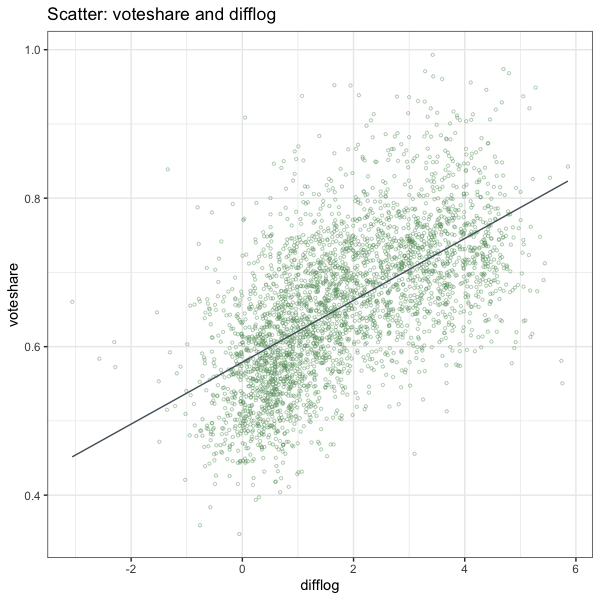
\includegraphics[scale=0.5]{q1_scatter.png}
		\end{figure}
		\item[$\bullet$] Generally speaking, difflog and voteshare are positively correlated.
		
		\newpage
		
		\item Save the residuals of the model in a separate object.	\\
		
		In regression model, residuals suggests the differences between the predict values and the true values. \\
		
		The formulation of residuals is: $ e_i = y_i - \hat{y_i}$ \\
		
		In this formulation: \\
		$e_i$ is residuals, $y_i$ is the reality value, and $\hat{y_i}$ is the value of the regression model. \\
		
		Below is the R code:
			\lstinputlisting[language=R, firstline=53, lastline=57]{PS03_answers_Chenxi.R}
		Below is the output in R studio: 
		\begin{verbatim}
			> str(q1_residuals) Named num [1:3193] -0.000423 -0.031684 -0.004551
			 0.038669 0.035529 ... 
			- attr(*, "names")= chr [1:3193] "1" "2" "3" "4" ...
			> summary(q1_residuals)     Min.   1st Qu.    Median    Mean   3rd Qu.   Max. 
			-0.268319 -0.053454 -0.003769  0.000000  0.047798  0.327488 
		\end{verbatim}
		
		\newpage
		
		\item Write the prediction equation. \\
		
		Because regression model in R is a list composed of coefficients, residuals, effects and many other elements. \\
		
		For coefficients, the first element is the intercept, and the second element is the slope. \\
		
		Below is the R code:
		\lstinputlisting[language=R, firstline=59, lastline=68]{PS03_answers_Chenxi.R}
		
		Below is the output in R studio:
		\begin{verbatim}
		[1] "voteshare = 0.58 + 0.04 * difflog"
		\end{verbatim}
	\end{enumerate}
	
\newpage

\section*{Question 2}
\noindent We are interested in knowing how the difference between incumbent and challenger's spending and the vote share of the presidential candidate of the incumbent's party are related.	\vspace{.25cm}
	\begin{enumerate}
			\item Run a regression where the outcome variable is \texttt{presvote} and the explanatory variable is \texttt{difflog}. \\
			
	Below is the R code:
	\lstinputlisting[language=R, firstline=70, lastline=75]{PS03_answers_Chenxi.R}

	\begin{table}[ht]
		\centering
		\caption{Abstract of Regression Model in Question 2}
		\begin{tabular}{lcccc}
			\toprule
			& Estimate & Std. Error & t value & Pr($>|t|$) \\
			\midrule
			(Intercept) & 0.507583 &0.003161 & 160.60 & <2e-16 *** \\
			difflog & 0.023837 & 0.001359 & 17.54 & <2e-16 *** \\
			\bottomrule
		\end{tabular} 
	\end{table}
	\begin{verbatim}
	---Signif. codes:  0 ‘***’ 0.001 ‘**’ 0.01 ‘*’ 0.05 ‘.’ 0.1 ‘ ’ 1
	
	Residual standard error: 0.1104 on 3191 degrees of freedom
	Multiple R-squared:  0.08795,	Adjusted R-squared:  0.08767 
	F-statistic: 307.7 on 1 and 3191 DF,  p-value: < 2.2e-16
	\end{verbatim}
		We can conclude from the results:
		\item[$\bullet$] F test p-value for the entire regression model is 2.2e-16, which is very close to 0, which means we have a very high confidence in rejecting the null hypothesis.. So at least one slope in regression model is not 0.
		\item[$\bullet$] F test p-value for the intercept and slope is both 2e-16,which is very close to 0, which means we have a very high confidence in rejecting the null hypothesis.. So the estimate of intercept and slope is not 0.
		\item[$\bullet$] The adjusted R-squared is 0.08767, which means that the fit of this model is very bad.
		
		\newpage
		
		\item Make a scatterplot of the two variables and add the regression line. \\
		
		Below is the R code:
		\lstinputlisting[language=R, firstline=77, lastline=84]{PS03_answers_Chenxi.R}
		\begin{figure}[h]
			\centering
			\caption{Scatter - Difflog and Presvote}
			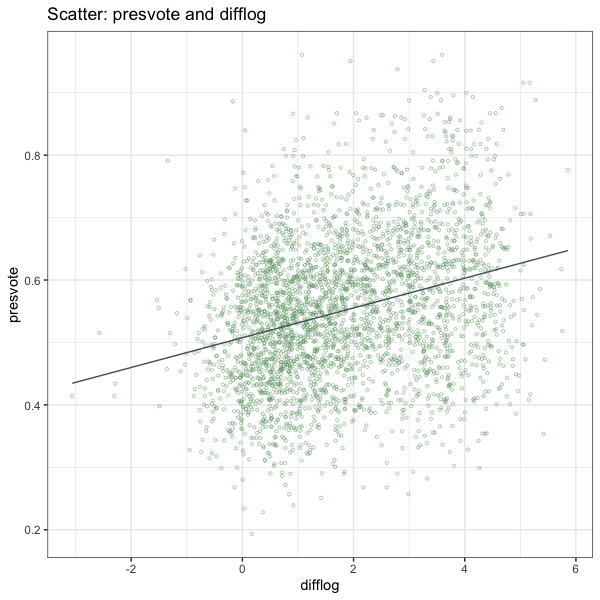
\includegraphics[scale=0.5]{q2_scatter.png}
		\end{figure}
		\item[$\bullet$] Generally speaking, difflog and voteshare are positively correlated.
		
		\newpage
		
		\item Save the residuals of the model in a separate object.	\\
		
		In regression model, residuals suggests the differences between the predict values and the true values. \\
		
		The formulation of residuals is: $ e_i = y_i - \hat{y_i}$ \\
		
		In this formulation: \\
		$e_i$ is residuals, $y_i$ is the reality value, and $\hat{y_i}$ is the value of the regression model. \\
		
		Below is the R code:
		\lstinputlisting[language=R, firstline=86, lastline=90]{PS03_answers_Chenxi.R}
		Below is the output in R studio: 
		\begin{verbatim}
		> str(q2_residuals) Named num [1:3193] 0.00561 0.03758 -0.05313 
		-0.05299 -0.04584 ... 
		- attr(*, "names")= chr [1:3193] "1" "2" "3" "4" ...
		> summary(q2_residuals)   Min.  1st Qu.   Median  Mean  3rd Qu.  Max.
		-0.321965 -0.074069 -0.001018  0.000000  0.071507  0.427435
		\end{verbatim}
		
		\newpage
		
		\item Write the prediction equation. 
		
		Because regression model in R is a list composed of coefficients, residuals, effects and many other elements. \\
		
		For coefficients, the first element is the intercept, and the second element is the slope. \\
		
		Below is the R code:
		\lstinputlisting[language=R, firstline=92, lastline=101]{PS03_answers_Chenxi.R}
		
		Below is the output in R studio:
		\begin{verbatim}
			[1] "presvote = 0.51 + 0.02 * difflog"
		\end{verbatim}
		\newpage
	\end{enumerate}
	
	\newpage	
\section*{Question 3}

\noindent We are interested in knowing how the vote share of the presidential candidate of the incumbent's party is associated with the incumbent's electoral success.
	\vspace{.25cm}
	\begin{enumerate}
		\item Run a regression where the outcome variable is \texttt{voteshare} and the explanatory variable is \texttt{presvote}. \\
		
		Below is the R code:
		\lstinputlisting[language=R, firstline=105, lastline=108]{PS03_answers_Chenxi.R}
		
		\begin{table}[ht]
			\centering
			\caption{Abstract of Regression Model in Question 3}
			\begin{tabular}{lcccc}
				\toprule
				& Estimate & Std. Error & t value & Pr($>|t|$) \\
				\midrule
				(Intercept) & 0.441330 &0.007599 & 58.08 & <2e-16 *** \\
				presvote & 0.388018 & 0.013493 & 28.76 & <2e-16 *** \\
				\bottomrule
			\end{tabular} 
		\end{table}
		\begin{verbatim}
		---Signif. codes:  0 ‘***’ 0.001 ‘**’ 0.01 ‘*’ 0.05 ‘.’ 0.1 ‘ ’ 1
		
		Residual standard error: 	0.08815 on 3191 degrees of freedom
		Multiple R-squared:  0.2058,	Adjusted R-squared:  0.2056 
		F-statistic:   827 on 1 and 3191 DF,  p-value: < 2.2e-16
		\end{verbatim}
		We can conclude from the results:
		\item[$\bullet$] F test p-value for the entire regression model is 2.2e-16, which is very close to 0, which means we have a very high confidence in rejecting the null hypothesis. So at least one slope in regression model is not 0.
		\item[$\bullet$] F test p-value for the intercept and slope is both 2e-16,which is very close to 0, which means we have a very high confidence in rejecting the null hypothesis. So the estimate of intercept and slope is not 0.
		\item[$\bullet$] The adjusted R-squared is 0.08815, which means that the fit of this model is very bad.
		
		\newpage
		
		\item Make a scatterplot of the two variables and add the regression line. 
		
		Below is the R code:
		\lstinputlisting[language=R, firstline=110, lastline=117]{PS03_answers_Chenxi.R}
		\begin{figure}[h]
			\centering
			\caption{Scatter - Voteshare and Presvote}
			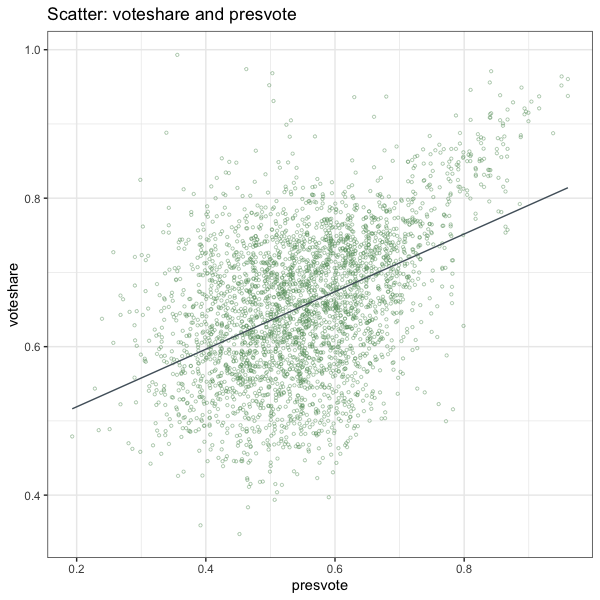
\includegraphics[scale=0.5]{q3_scatter.png}
		\end{figure}
		\item[$\bullet$] Generally speaking, voteshare and presvote are positively correlated.
		
		\newpage
		
		\item Write the prediction equation. \\
		
		Because regression model in R is a list composed of coefficients, residuals, effects and many other elements. \\
		
		For coefficients, the first element is the intercept, and the second element is the slope. \\
		
		Below is the R code:
		\lstinputlisting[language=R, firstline=119, lastline=128]{PS03_answers_Chenxi.R}
		
		Below is the output in R studio:
		\begin{verbatim}
			[1] "voteshare = 0.44 + 0.39 * presvote"
		\end{verbatim}
		
		\newpage	
		
	\end{enumerate}
	
\newpage	
\section*{Question 4}
\noindent The residuals from part (a) tell us how much of the variation in \texttt{voteshare} is $not$ explained by the difference in spending between incumbent and challenger. The residuals in part (b) tell us how much of the variation in \texttt{presvote} is $not$ explained by the difference in spending between incumbent and challenger in the district.
	\begin{enumerate}
		\item Run a regression where the outcome variable is the residuals from Question 1 and the explanatory variable is the residuals from Question 2.\\
		
		Below is the R code:
		\lstinputlisting[language=R, firstline=130, lastline=135]{PS03_answers_Chenxi.R}
		
		\begin{table}[ht]
			\centering
			\caption{Abstract of Regression Model in Question 4}
			\begin{tabular}{lcccc}
				\toprule
				& Estimate & Std. Error & t value & Pr($>|t|$) \\
				\midrule
				(Intercept) & -1.942e-18 &1.299e-03 & 0.00 & 1 \\
				q2residuals & 2.569e-01 & 1.176e-02 & 21.84 & <2e-16 *** \\
				\bottomrule
			\end{tabular} 
		\end{table}
		\begin{verbatim}
			---Signif. codes:  0 ‘***’ 0.001 ‘**’ 0.01 ‘*’ 0.05 ‘.’ 0.1 ‘ ’ 1
			
			Residual standard error: 	0.0733 on 3191 degrees of freedom
			Multiple R-squared:  0.13,	Adjusted R-squared:  0.1298 
			F-statistic:   477 on 1 and 3191 DF,  p-value: < 2.2e-16
		\end{verbatim}
		We can conclude from the results:
		\item[$\bullet$] F test p-value for the entire regression model is 2.2e-16, which is very close to 0, which means we have a very high confidence in rejecting the null hypothesis. So at least one slope in regression model is not 0.
		\item[$\bullet$] F test p-value for the intercept and slope is correspondingly 1 and 2e-16,the first one didn't pass the statistics test, which means the intercept is 0. And the second one is very close to 0,  which means we have a very high confidence in rejecting the null hypothesis. So the estimate of slope is not 0.
		\item[$\bullet$] The adjusted R-squared is 0.1298, which means that the fit of this model is very bad.
		
		\newpage
		
		\item Make a scatterplot of the two residuals and add the regression line. \\
		
		Below is the R code:
		\lstinputlisting[language=R, firstline=110, lastline=117]{PS03_answers_Chenxi.R}
		\begin{figure}[h]
			\centering
			\caption{Scatter - q1residuals and q2residuals}
			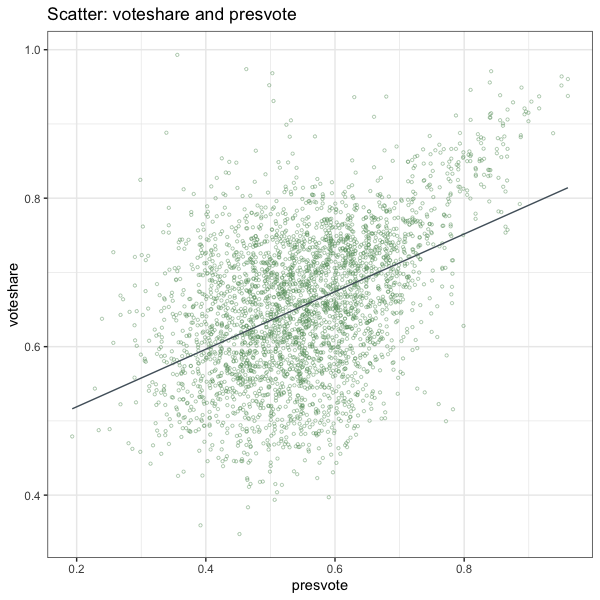
\includegraphics[scale=0.5]{q3_scatter.png}
		\end{figure}
		\item[$\bullet$] Generally speaking, q1residuals and q2residuals are positively correlated.
		
		\newpage
			
		\item Write the prediction equation.
		
		Because regression model in R is a list composed of coefficients, residuals, effects and many other elements. \\
		
		For coefficients, the first element is the intercept, and the second element is the slope. \\
		
		Below is the R code:
		\lstinputlisting[language=R, firstline=146, lastline=155]{PS03_answers_Chenxi.R}
		
		Below is the output in R studio:
		\begin{verbatim}
			[1] "q1_residuals = 0 + 0.26 * q2_residuals"
		\end{verbatim}
		
	\end{enumerate}
	
	\newpage	

\section*{Question 5}
\noindent What if the incumbent's vote share is affected by both the president's popularity and the difference in spending between incumbent and challenger? 
	\begin{enumerate}
		\item Run a regression where the outcome variable is the incumbent's \texttt{voteshare} and the explanatory variables are \texttt{difflog} and \texttt{presvote}.	\\
		
		Below is the R code:
		\lstinputlisting[language=R, firstline=157, lastline=162]{PS03_answers_Chenxi.R}
		
		\begin{table}[ht]
			\centering
			\caption{Abstract of Regression Model in Question 5}
			\begin{tabular}{lcccc}
				\toprule
				& Estimate & Std. Error & t value & Pr($>|t|$) \\
				\midrule
				(Intercept) & 0.4486442 &0.0063297 & 70.88 &  <2e-16 *** \\
				difflog & 0.0355431 & 0.0009455& 37.59 & <2e-16 *** \\
				presvote & 0.2568770 & 0.0117637 & 21.84 & <2e-16 *** \\
				\bottomrule
			\end{tabular} 
		\end{table}
		\begin{verbatim}
			---Signif. codes:  0 ‘***’ 0.001 ‘**’ 0.01 ‘*’ 0.05 ‘.’ 0.1 ‘ ’ 1
			
			Residual standard error: 	0.0739 on 3190 degrees of freedom
			Multiple R-squared:  0.4496	Adjusted R-squared:  0.4493 
			F-statistic:   1303 on 2 and 3190 DF,  p-value: < 2.2e-16
		\end{verbatim}
		We can conclude from the results:
		\item[$\bullet$] F test p-value for the entire regression model is 2.2e-16, which is very close to 0, which means we have a very high confidence in rejecting the null hypothesis. So at least one slope in regression model is not 0.
		\item[$\bullet$] F test p-value for the intercept and slope is both 2e-16, which is very close to 0,  which means we have a very high confidence in rejecting the null hypothesis. So the estimate of slope and intercept is not 0.
		\item[$\bullet$] The adjusted R-squared is 0.4493, which means that the fit of this model is average.
		
		\newpage
		
		\item Write the prediction equation. \\ 
		
		Because regression model in R is a list composed of coefficients, residuals, effects and many other elements. \\
		
		For coefficients, the first element is the intercept, and the second element is the slope. \\
		
		Below is the R code:
		\lstinputlisting[language=R, firstline=164, lastline=176]{PS03_answers_Chenxi.R}
		
		Below is the output in R studio:
		\begin{verbatim}
			[1] "voteshare = 0.45 + 0.04 * difflog + 0.26 * presvote"
		\end{verbatim}

		\item What is it in this output that is identical to the output in Question 4? Why do you think this is the case? \\
		
		I found that the residuals in question 4's regression model is the same as the one in question 5. We can check that in R code and box plot. Below is the R code: \\
		\lstinputlisting[language=R, firstline=178, lastline=194]{PS03_answers_Chenxi.R}
		
		\begin{figure}[h]
			\centering
			\caption{Boxplot - Residuals in Question 4 and 5}
			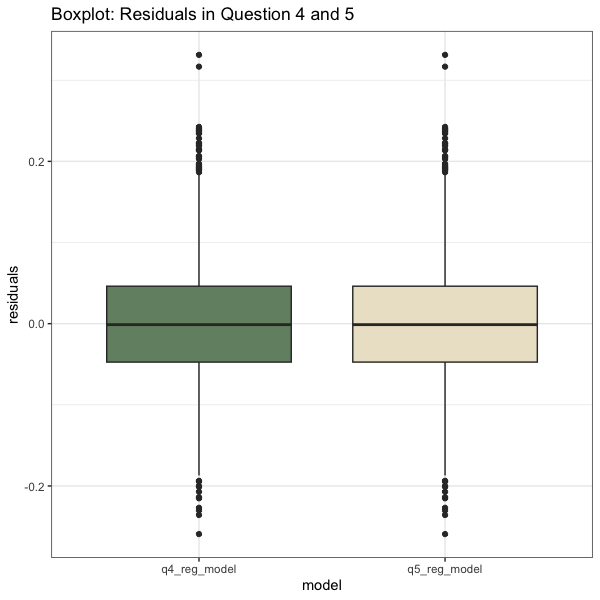
\includegraphics[scale=0.5]{q5_boxplot.png}
		\end{figure}
		
				If two regression model's residuals is the same, we can conclude that:
		
		\item[$\bullet$] The homoskedasticity assumption is met: the residual variances of the two models are similar at different levels of the explanatory variables.
		\item[$\bullet$]The model fits the data well: The presence of homoscedasticity may indicate that the model fits the data well because it meets the basic assumptions of linear regression.
		\item[$\bullet$]Reliability of model comparisons and interpretations: Model comparisons and interpretation of model results can be made more reliably if the residuals of two models are the same.
		
	\end{enumerate}

\end{document}
